\documentclass[a4paper,10pt]{article}
\usepackage[utf8]{inputenc}
\usepackage{natbib}
\usepackage{graphicx}% Include figure files
\usepackage{amsmath}


\newcommand{\inblue}[1]{{\color{blue}#1}}
\newcommand{\inred}[1]{{\color{red}#1}}

%opening
\title{Coherence vortices in the Cross Spectral Density. Something to consider in diffraction and imaging?}
\author{Manuel Sanchez del Rio$^1$, David Paganin$^2$}

\begin{document}

\maketitle

\begin{abstract}

\end{abstract}

\section{What is the Cross Spectral Density (CSD)?}

It is the function that fully describes the coherence properties of a synchrotron beam. It measures the correlation of the electric disturbance between two points,

\begin{equation}
W(x_1,y_1,x_2,y_2,z,\omega) = 
\langle E^{*}(x_1,y_1,z,\omega) E(x_2,y_2,z,\omega)\rangle.
\end{equation}

The CSD quantifies the two-point correlation properties of a partially coherent statistically stationary source \cite{mandel_wolf}. 
It is the input input needed to properly model any subsequent x-ray data obtained by streaming such CSD through subsequent optical elements, samples, and detector.

Recall that the cross-spectral density $W$, spectral density $S$ (intensity) and spectral degree of coherence (normalized CSD) $\mu$ are related by 
\begin{equation}
S(r_1,\omega) = W(r_1,r_1,\omega) 
\end{equation}

\begin{equation}
W(r_1,r_2,\omega)=\sqrt{S(r_1,\omega)}\sqrt{S(r_2,\omega)}\mu(r_1,r_2,\omega)
\end{equation}

In this work, we consider the role played by the phase of CSD

\begin{equation}\label{phase_of_W}
\Phi(x_1,y_1,x_2,y_2,z,\omega)=\arg[W(x_1,y_1,x_2,y_2,z,\omega)]
\end{equation}

It governs the position of Young-type interference fringes formed when the disturbance from two different spatial points is combined. It influences the detected intensity in both imaging and non-imaging experiments.






\section{What is a coherence vortex?}


%\begin{figure}\label{loss_of_fringe_visibility}
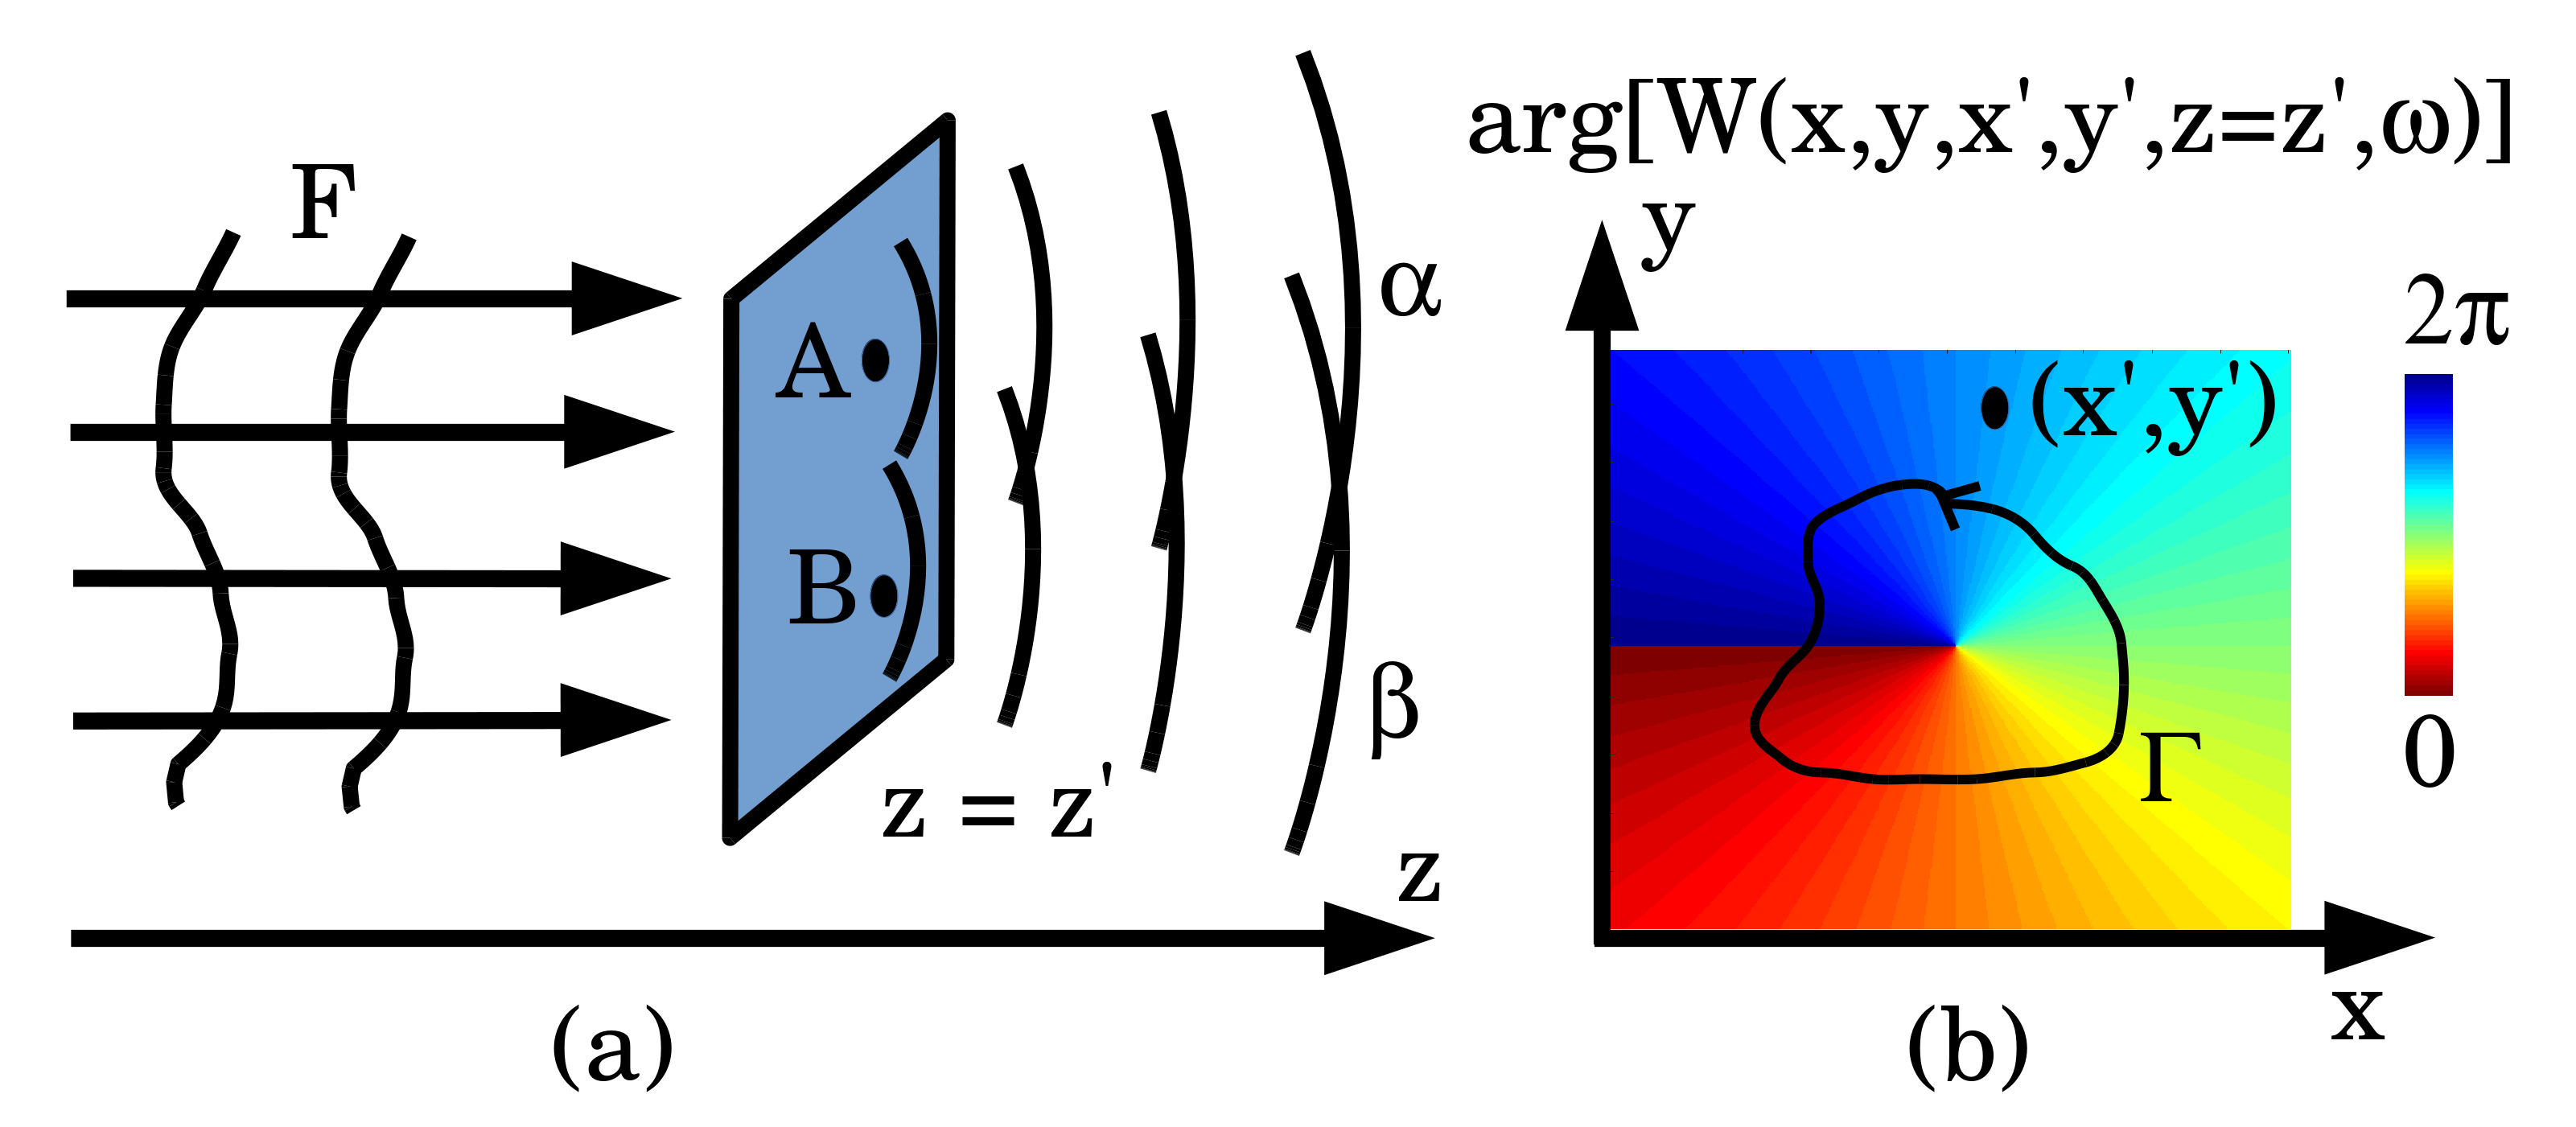
\includegraphics[width=1\textwidth]{Figures/coherence_vortex.png}
%\end{figure}
The CSD is a single-valued function, but its phase $\Phi$ will in general be multi-valued. Indeed, since the phase of a complex number is only defined modulo $2\pi$ radians, it may wind by an integer multiple of $2\pi$ in the following manner \cite{GburVisser2003}: 
\begin{equation}
\label{phase_of_W_winding}
\oint_{\Gamma} d\Phi(x_1,y_1,x_2,y_2,z,\omega)=2\pi m.
\end{equation}
Here, $\Gamma$ is any smooth closed curve as seen in the figure, $m$ is an integer and $d\Phi$ is the increment in $\Phi$ corresponding to an infinitesimal line segment of $\Gamma$.
{\bf A non-zero $m$ indicates the presence of non-trivial topology in the phase of the CSD, thus a coherence vortex \cite{GburVisser2003} is present}.  It can be recognized in the false color maps of the phase at the positions where at least three colors meet.

\section{What do a coherence vortex imply?}

The existence of any {\em one} circuit $\Gamma$ for which $m$ is non-zero around a point A, implies the presence of a manifold of points in $(x_A,y_A,x_B,y_B,z,\omega)$-space, at each of which $W$ vanishes. These nodal points in $W$ exhibit {\bf complete destructive interference of coherence}. 

If one has a point scatterer at $A$ and another point scatterer at $B$, the radiation scattered from both points overlap, but no interference fringes would be observed (curve 1).


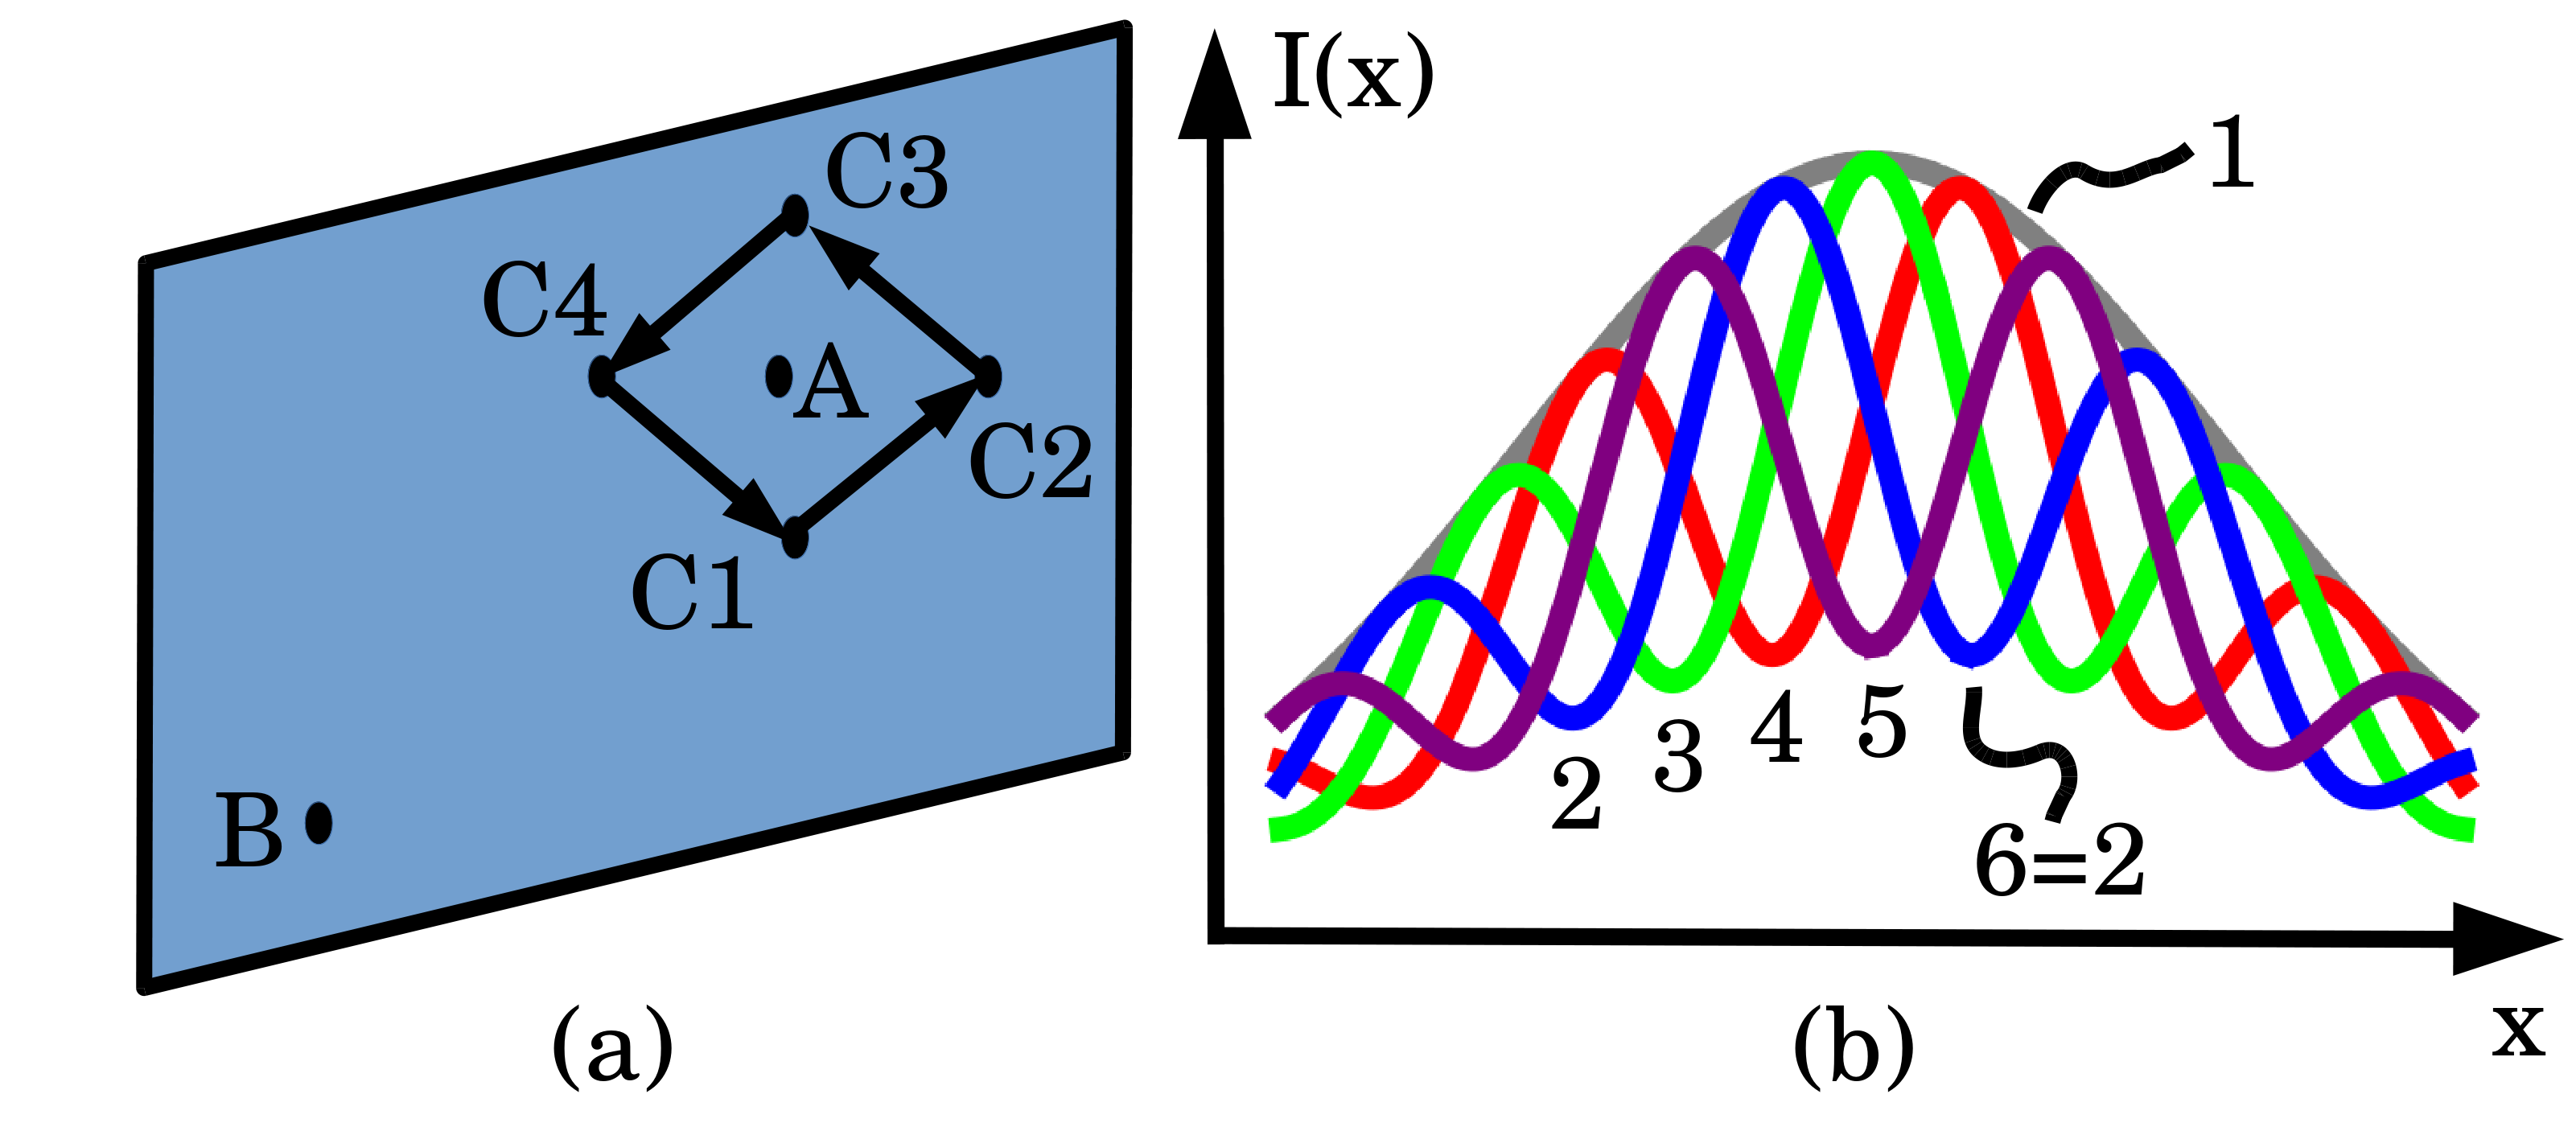
\includegraphics[width=0.7\textwidth]{Figures/Anholonomy.png}

 
Let us perform a sequence of Young-type interference experiments, where the pinhole at $B$ is kept fixed, while the pinhole at $C1$ is moved through the cycle of locations $C1$ (curve 2), $C2$ (curve 3), $C3$ (curve 4), $C4$ (curve 5) and finally back to $C1$ (curve 6 = curve 2). If one traces the evolution of the intensity maxima associated with the sequence of Young-type interferograms in curves 2 to 6, the physical meaning of $m$ becomes clear: during the cycle, if $m=1$ then the maxima of the interferogram will ``ratchet'' to the right by one fringe during the cycle. If $m=-1$ they would instead ratchet to the left by one fringe during the cycle.  For general $m$, the fringes would ratchet to the right (left) by $|m|$ fringes, if $m$ is positive (negative).

This is an example of a propagated ($z$=5~m) CSD built using 20 coherent modes. The red circle marks the point $D$ and the map shows $\mathcal{\Phi}(x,y)=\arg[W(x,y,x_D,y_D]$. The black circle is positioned on a vortex. 
 

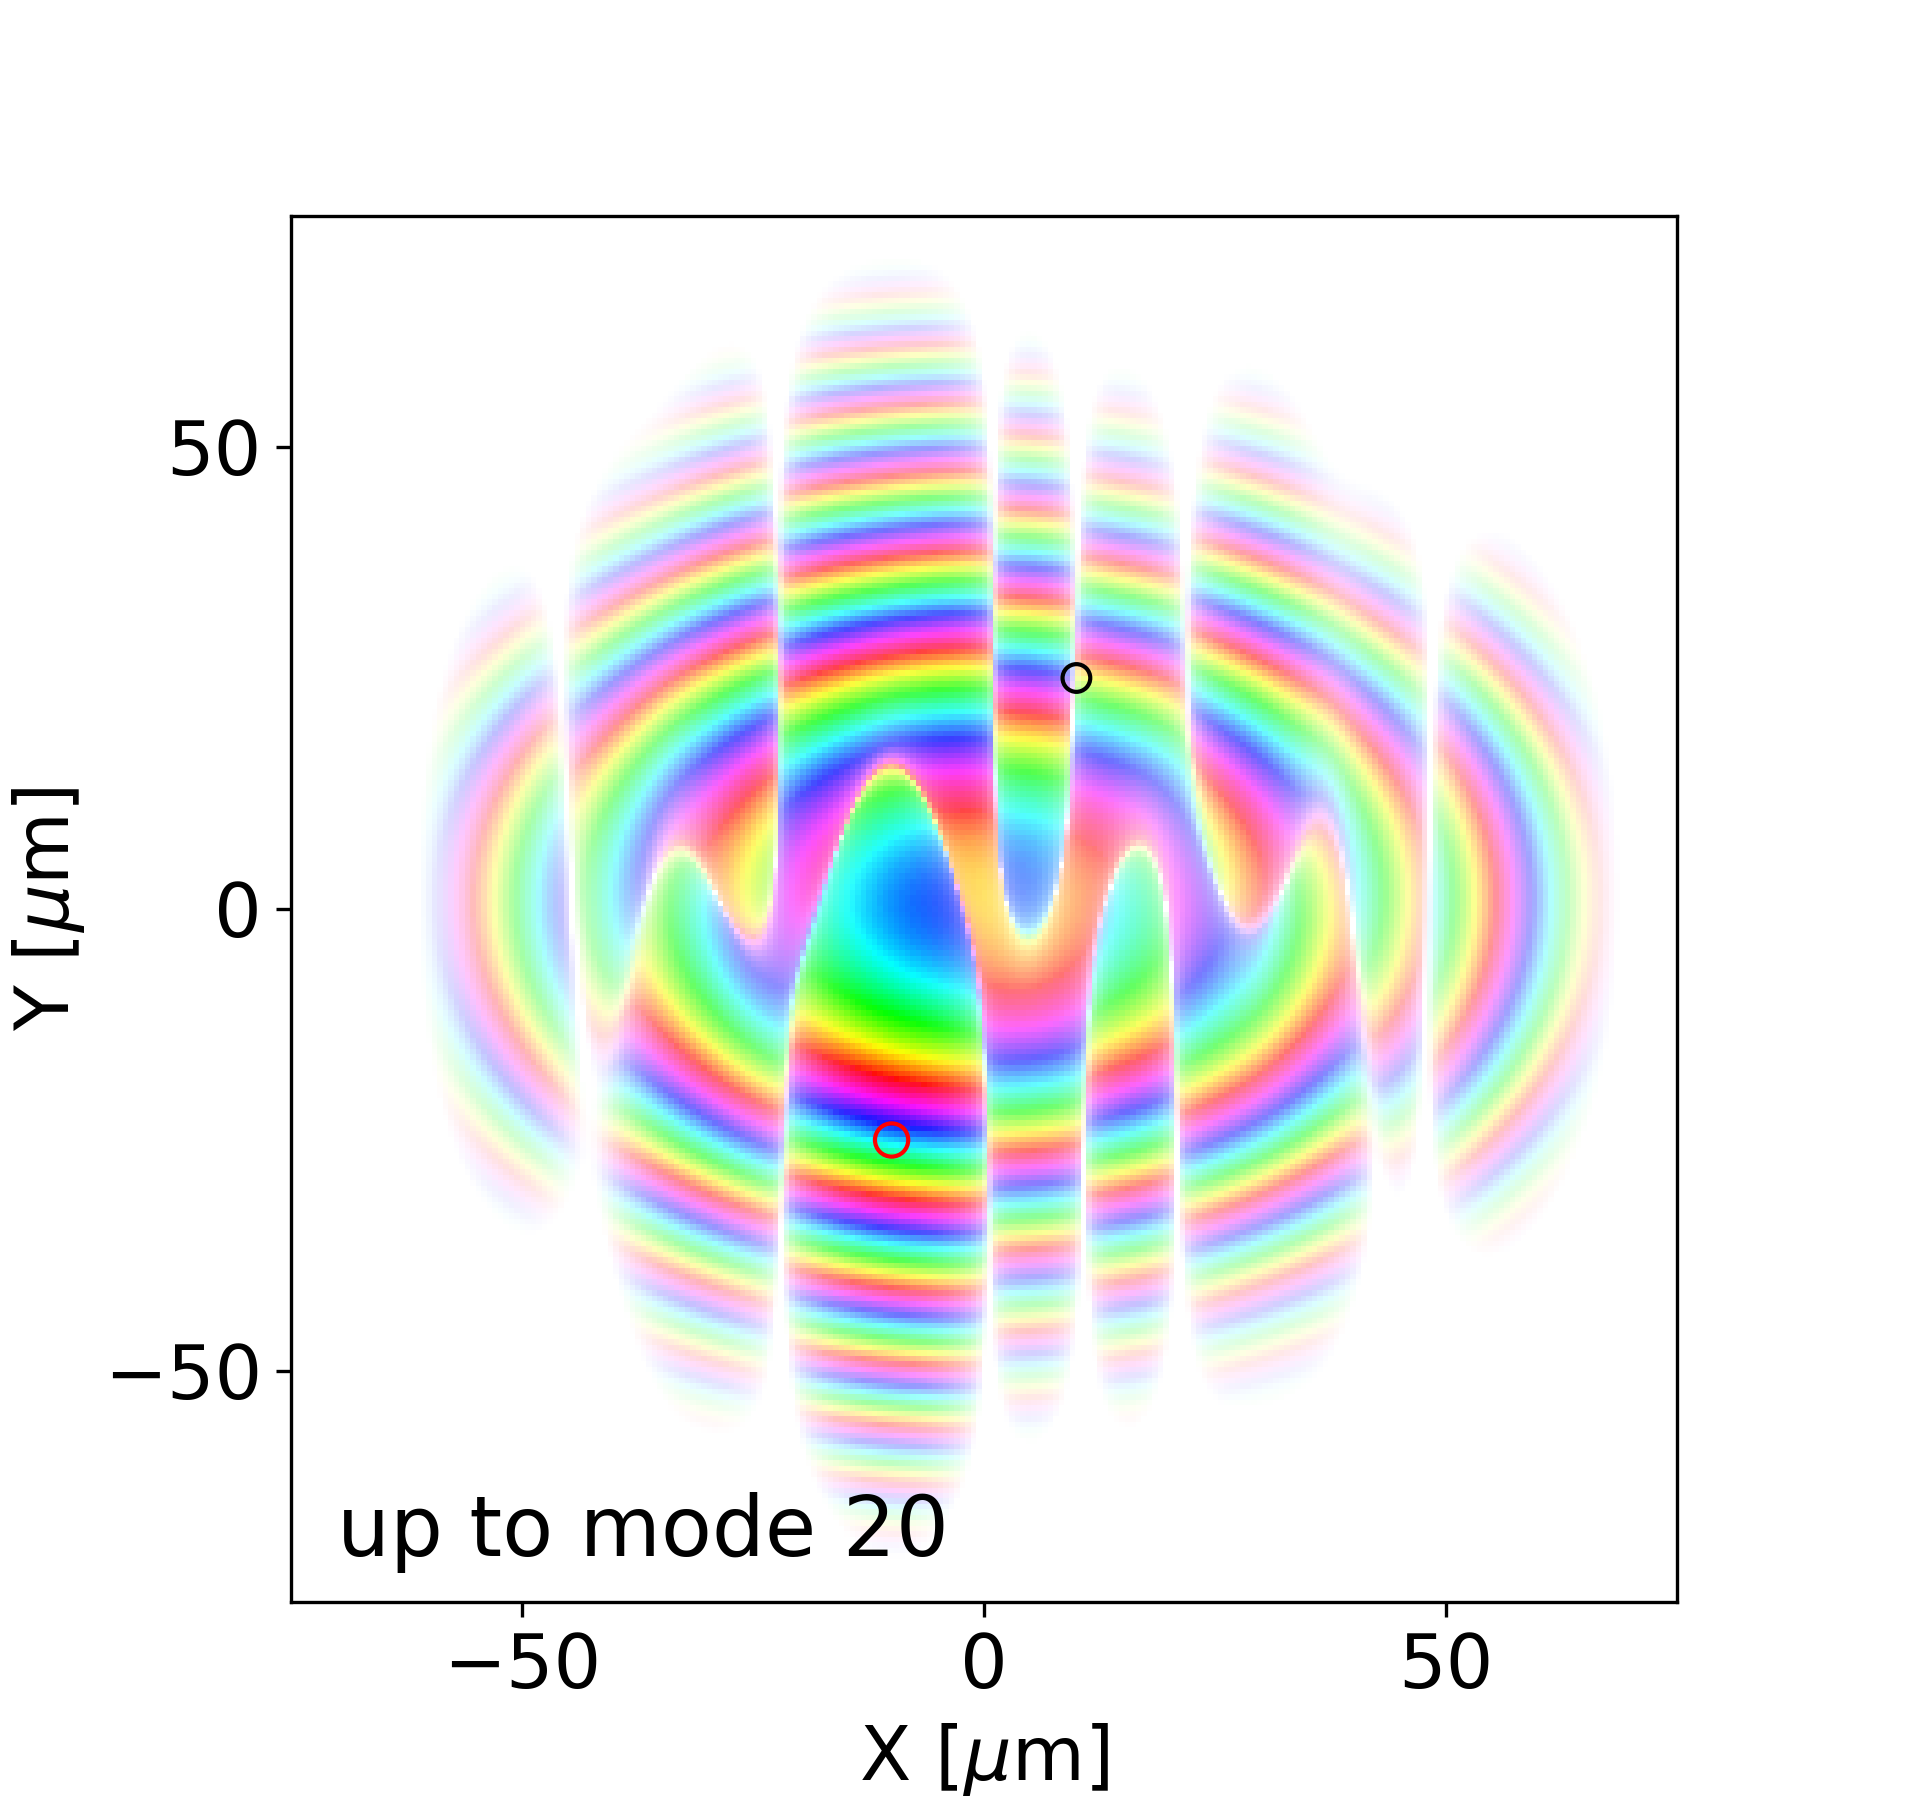
\includegraphics[width=0.7\textwidth]{FiguresPoster/interference_D_uptomode0020_csd.png}


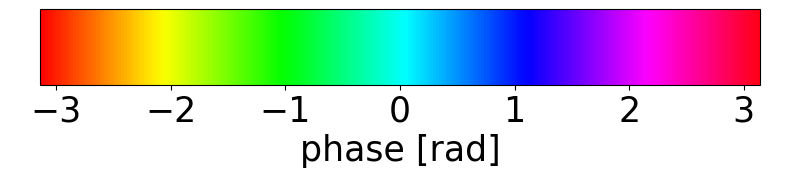
\includegraphics[width=0.7\textwidth]{Figures/colorbar.png}



\section{Do we expect coherence vortices in our synchrotron beams}

{\bf Yes. As far as the beam is partial coherent, like for the EBS and any other storage ring-based synchrotron source, there are coherence vortices}. Only fully coherent wavefronts ($W=cte$) and fully incoherent beams ($W=0$) do not present vortices. The number of vortices depend on the coherent fraction. More coherence imply less vortices, but their effect is more visible in a potential experiment. 

We present here a theoretical-numeric study  of the vortices in a synchrotron beam to be produced by EBS. {\bf We find correlation singularities in the CSD computed by a realistic x-ray undulator model, together with an associated speckled CSD structure}.


\section{How to calculate the CSD and its phase to look for vortices?}

We use COMSYL \cite{glass} to calculate the CSD expansion  in coherent modes, in the form:


\begin{equation}
W(\vec{r_1}, \vec{r_2}, \omega)
=
\sum_m
\lambda_m(\omega)
\phi_m^*(\vec{r_1},\omega)
\phi_m(\vec{r_2}, \omega).
\end{equation}

We analyzed the case if a U18 undulator at 17 keV placed at the EBS-ESRF storage ring. We need about 1000 modes to represent 97.9\% of the intensity. The occupation of the first coherent mode is 2.8\% (coherent fraction).  Later on, the beamline optics will reduce the number of modes down to a couple of modes with a subsequent reduction of intensity. 

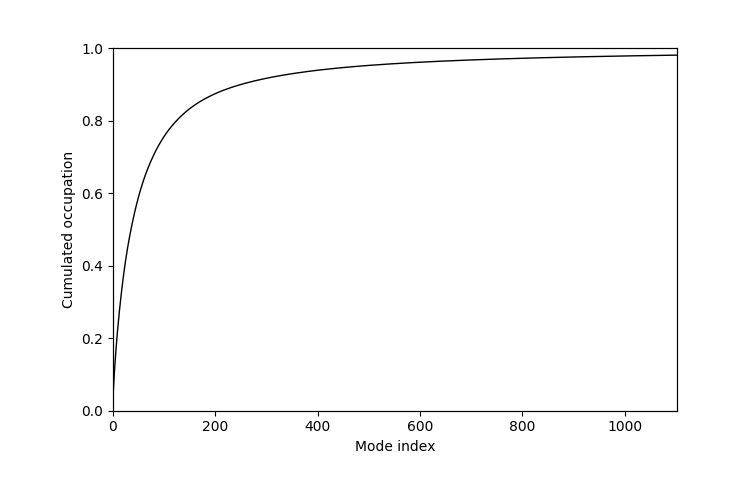
\includegraphics[width=0.6\textwidth]{Figures/vx_cumulated.png}

The total intensity (spectral density) at the source plane ($z$=0) is: 

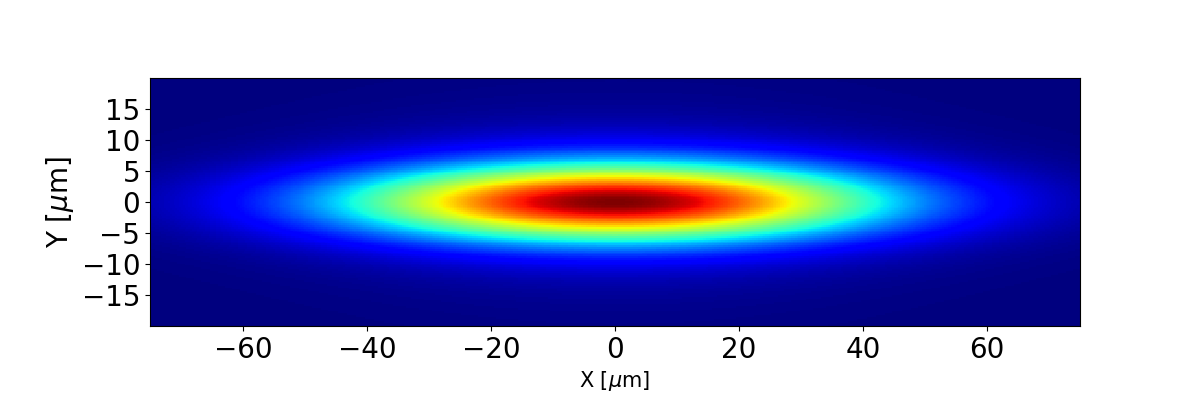
\includegraphics[width=0.85\textwidth]{Figures/spectral_density_upto1099.png}

The extension of the first coherent mode is:

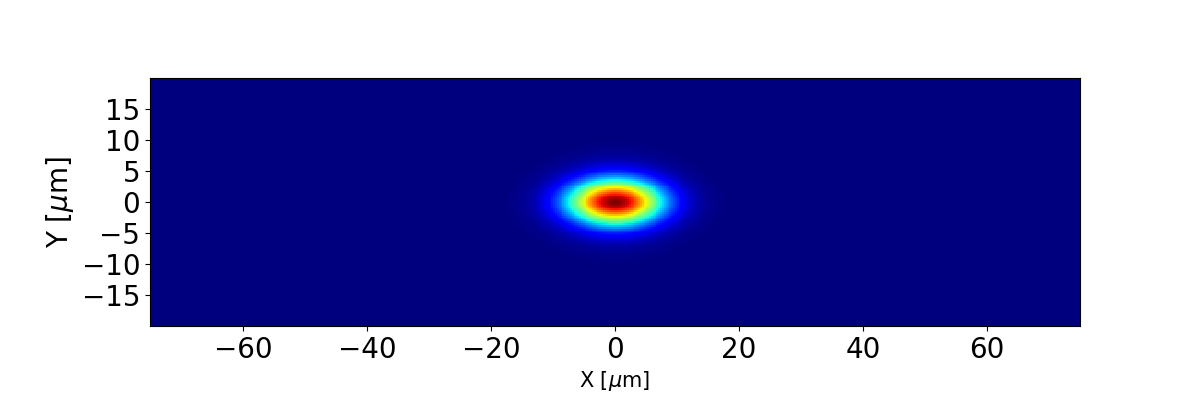
\includegraphics[width=0.85\textwidth]{Figures/spectral_density_upto0.png}

In a beamline some optical elements (ideal reflectors, ideal focusing elements) do not alter the occupation spectrum of the modes. They are non-absorbing or conservative elements in the sense of Smith-Helmholtz invariant. However, if an optical element remove photons from the beam, or ``cuts'' intensity, then its effect is different on the different modes. The new transformed ``modes'' can be used to build the CSD, but they cannot be considered coherent modes as they are not longer an orthonormal basis for expanding the CSD. A new coherent mode decomposition could be calculated on the transmitted CSD in order to obtain the new coherent modes. In the case of slits or pinholes centered on the optical axis, the lower coherent modes localised near the center of the beam axis will propagate, whereas the higher coherent modes that extend far from the axis will be absorbed. This will push of the occupation spectrum to the lower modes with a consequent increase of coherence fraction but an obvious decrease of the spectral density (total intensity).  



We then fix a point (e.g., ``A'') and compute the phase of the CSD up to a given mode $N$. 

\begin{equation}\label{phase_of_W}
\Phi_A(x_1,y_1;z=0,\omega)= %\arg[W(x_1,y_1,x_A,y_A;z,\omega)]=\arg[
\sum_{m=0}^{N-1} \lambda_m(\omega)
\phi_m^*(x_1,y_1,\omega)
\phi_m(x_A,y_A, \omega)]
\end{equation}

By selecting different points (A,B,C) and calculating the phase up to a given mode index we observe how vortices appear. They are manifested as points where three colors merge.  Indeed, the CSD phase possess a network of branch lines around which it has a non-zero winding number, and at which the CSD vanishes.

\begin{center}
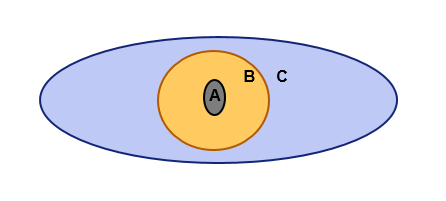
\includegraphics[width=0.25\textwidth]{Figures/eye}

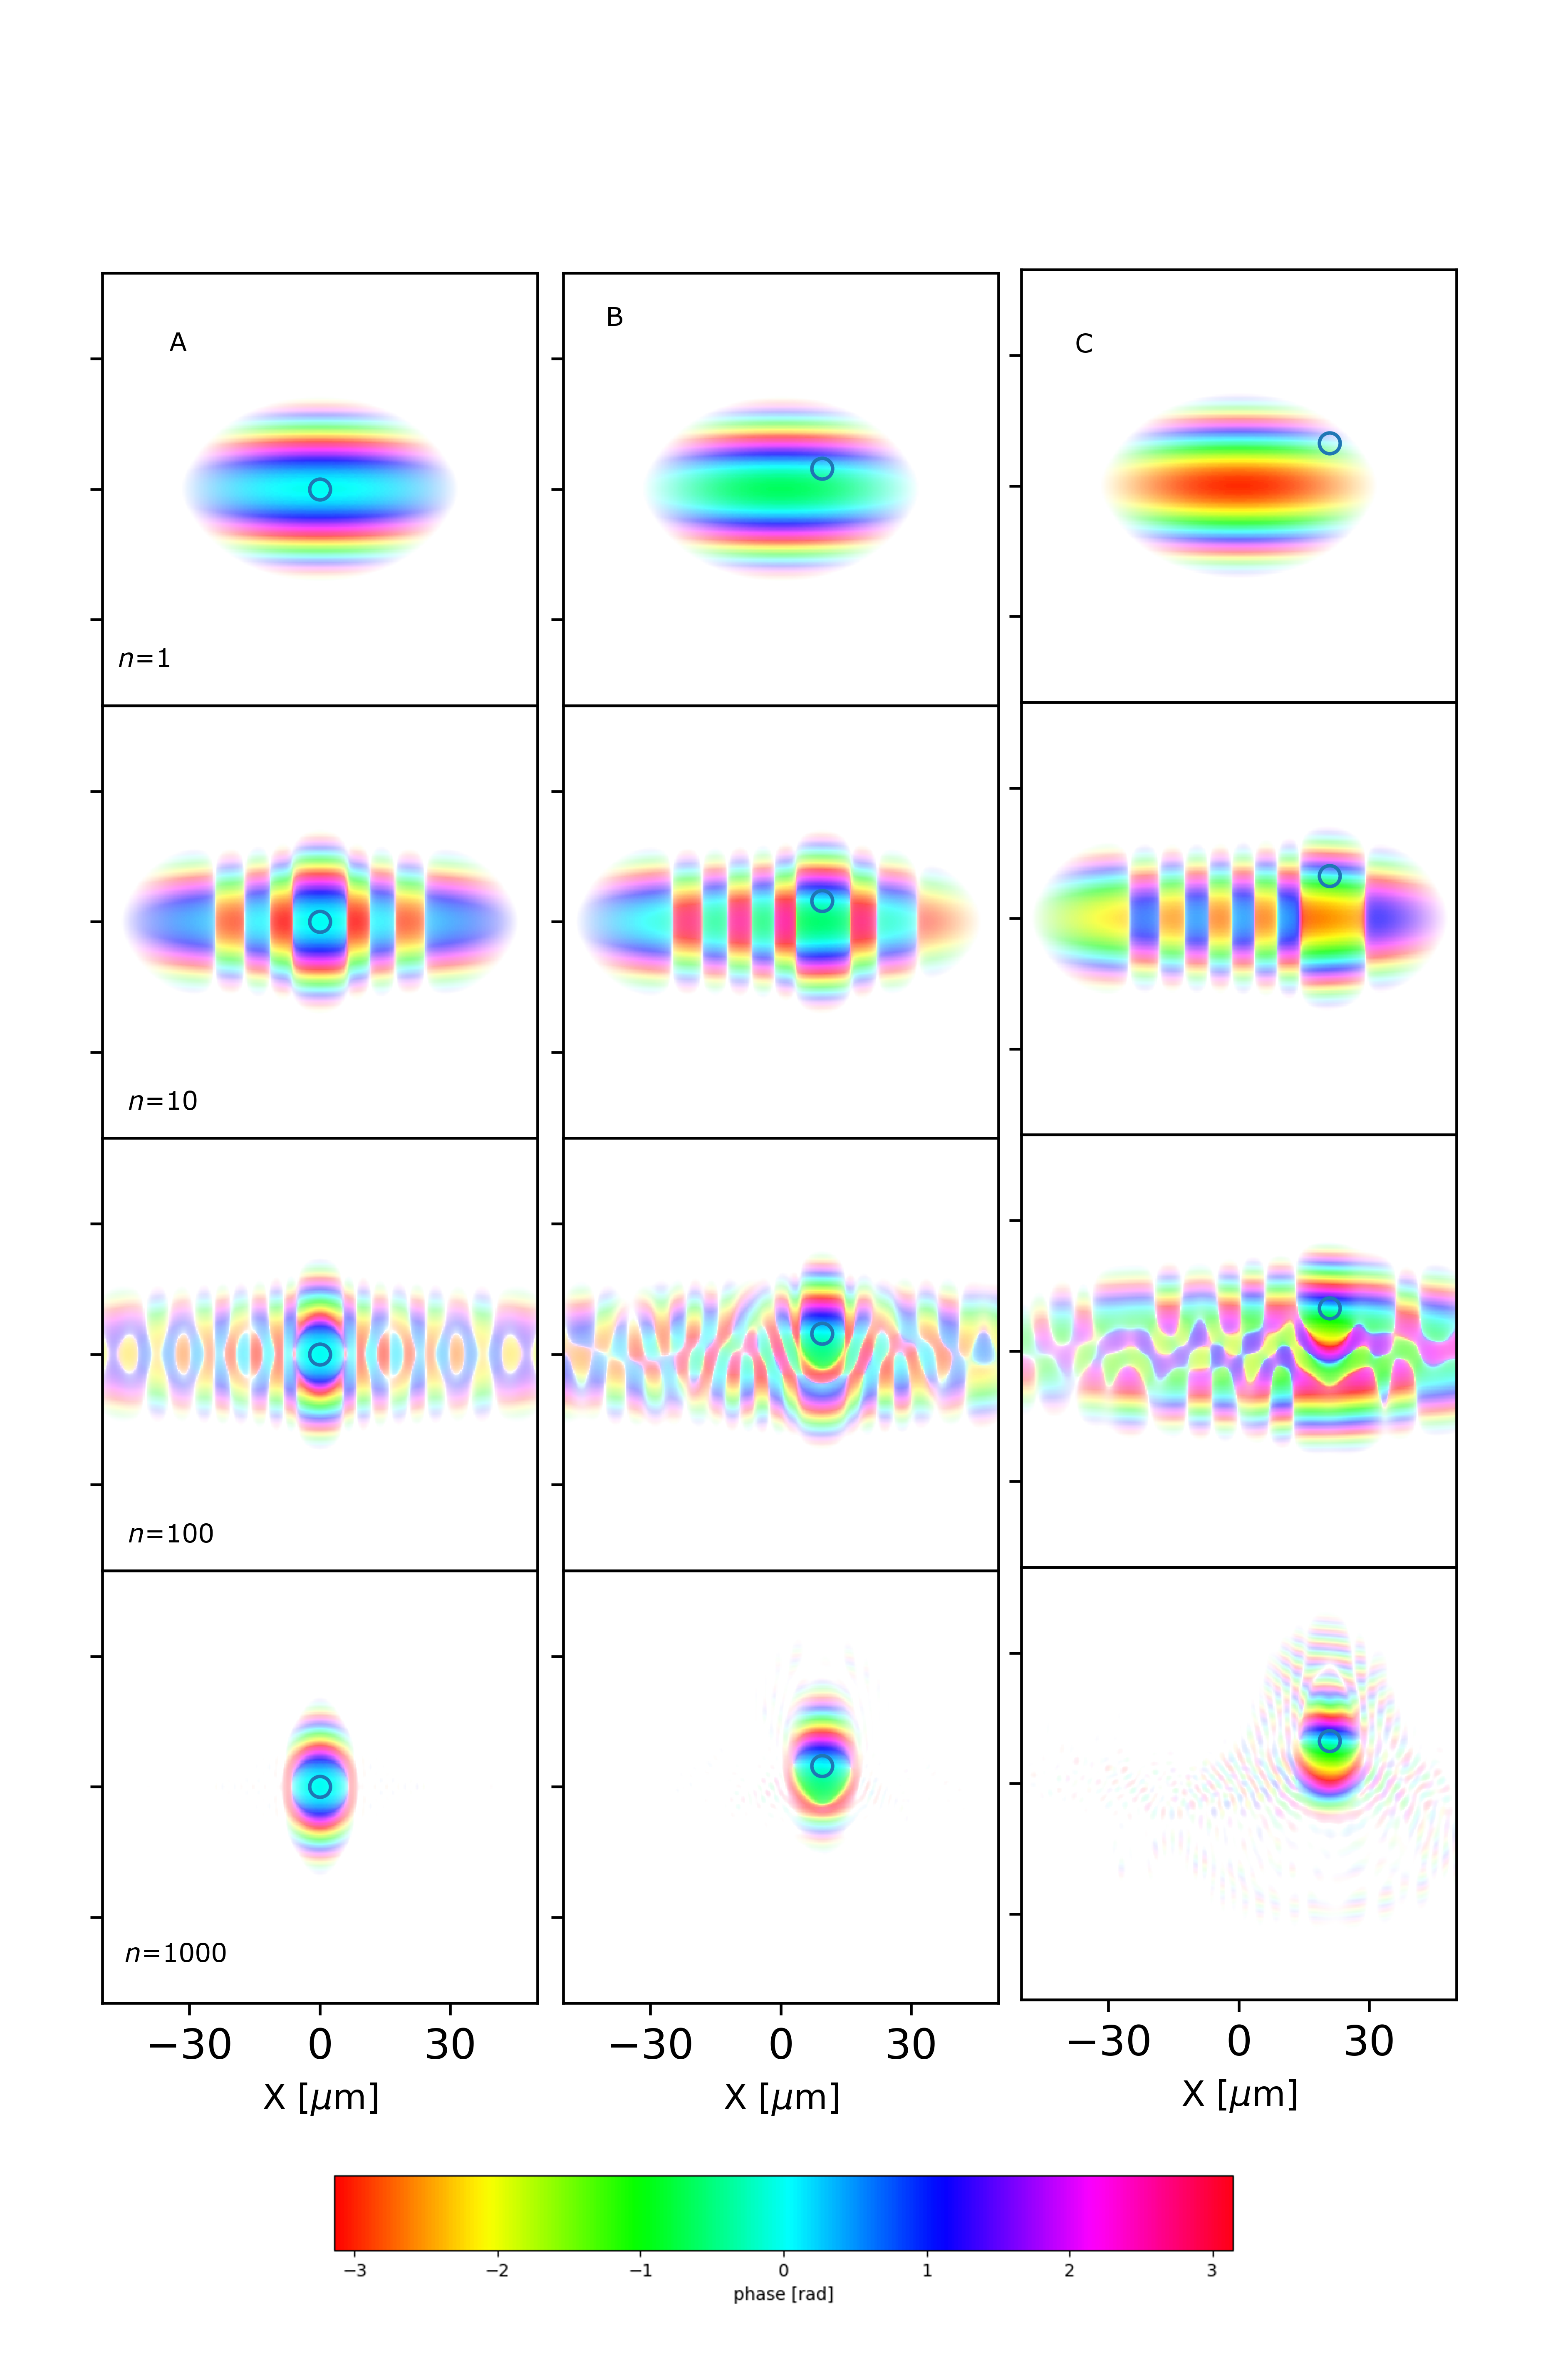
\includegraphics[width=0.95\textwidth]{Figures/vx_id16a_ABC.png}
\end{center}
 
 
 \section{Propagated vortices and their effect of reduction of visibility in a Young-like experiment}

We analyze here a Young-like experiment. The phase of the CSD (left column) has been calculated in a plane at $z$=5~m by fixing one point (the center of the red circle). This is the first pinhole, the second one is the black circle. We then propagate the outcoming radiation to an image plane at $z$=35~m, where the intensity os recorded (right column). One can observe: 

\begin{itemize}
\item The first coherent mode (complete coherence) does not present vortices and produce an image pattern with high visibility of interference fringes (row 1)
\item Adding more coherent modes (up to mode 3) makes the beam partially coherent and reduces the fringes visibility. 
\item Next mode (up to mode 4) introduces a vortex in the black pinhole, with a subsequent decrease of visibility. Next mode 5 (not shown) does not change the situation. 
\item When the 6th mode is added, the vortex is pushed out of the black pinhole, and visibility is partially recovered. 
\item This situation repeats several times as one increases the number of modes that contribute to the CSD. For example, the CSD built with modes up to 18 does not present a vortex in the red pinhole, but up to mode 20 it does. Increasing the number of modes used for building the CSD makes an the beam less and less coherent, and the fringes visibility is then lost, about the 99th mode.

\end{itemize}

\begin{center}
 \includegraphics[width=0.5\textwidth]{Figures/interference.png}
 \end{center}

\section{conclusion}

\begin{itemize}
\item Coherence vortices will exist in most non-trivial x-ray fields like synchrotron sources. An understanding of their existence will deepen our understanding of imaging and diffraction data obtained at EBS
\item Such coherence vortices influence the images that one takes, in ways that may lead to misleading results if one simply ignores their existence
\end{itemize}
 
 
 
 
 
 
 
 
 
\bibliographystyle{plain}
\bibliography{iucr}

\end{document}
